\documentclass[tikz,border=5pt]{standalone}
\usepackage{fontspec}
\setmainfont{Times New Roman}
\usepackage{unicode-math}
\setmathfont{Cambria Math}
\usetikzlibrary{shapes.geometric,shapes.misc,positioning,fit,backgrounds,arrows.meta,calc}

\begin{document}
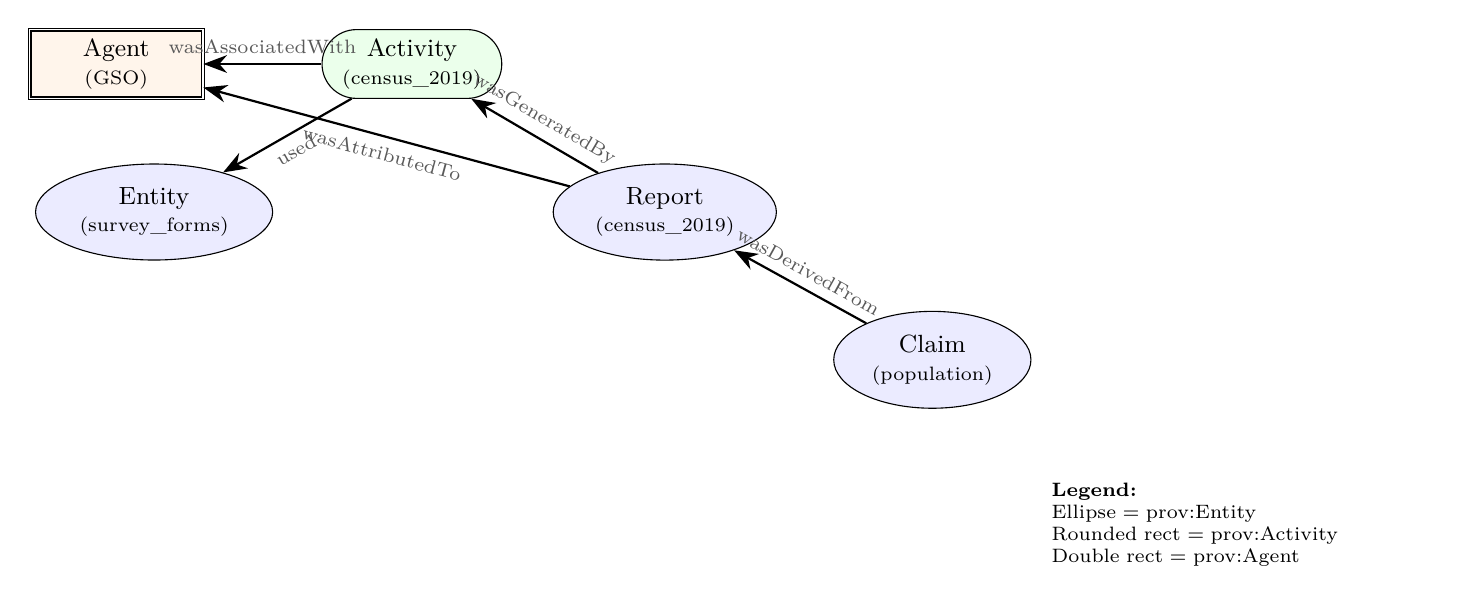
\begin{tikzpicture}[
    node distance=1.0cm and 1.5cm,
    entity/.style={ellipse, draw, minimum width=2.2cm, minimum height=0.8cm, align=center, font=\small},
    activity/.style={rounded rectangle, draw, minimum width=2.2cm, minimum height=0.8cm, align=center, font=\small},
    agent/.style={rectangle, draw, double, minimum width=2.2cm, minimum height=0.8cm, align=center, font=\small},
    arrow/.style={-{Stealth[length=3mm]}, thick},
    lbl/.style={font=\scriptsize, text=gray!70!black, sloped},
]

% Nodes
\node[entity, fill=blue!8] (claim) {Claim\\[-1pt]\scriptsize(population)};
\node[entity, fill=blue!8, above left=of claim] (report) {Report\\[-1pt]\scriptsize(census\_2019)};
\node[activity, fill=green!8, above left=of report] (census) {Activity\\[-1pt]\scriptsize(census\_2019)};
\node[agent, fill=orange!8, left=of census] (gso) {Agent\\[-1pt]\scriptsize(GSO)};
\node[entity, fill=blue!8, below left=of census] (survey) {Entity\\[-1pt]\scriptsize(survey\_forms)};

% Relations
\draw[arrow] (claim) -- node[lbl, above] {wasDerivedFrom} (report);
\draw[arrow] (report) -- node[lbl, above] {wasGeneratedBy} (census);
\draw[arrow] (report) -- node[lbl, below] {wasAttributedTo} (gso);
\draw[arrow] (census) -- node[lbl, above] {wasAssociatedWith} (gso);
\draw[arrow] (census) -- node[lbl, below] {used} (survey);

% Legend
\node[below right=1.0cm and 0.5cm of claim, font=\scriptsize, align=left, text width=5cm] {
    \textbf{Legend:}\\
    Ellipse = prov:Entity\\
    Rounded rect = prov:Activity\\
    Double rect = prov:Agent
};

\end{tikzpicture}
\end{document}
